% Preprint template for the BIND Lightcone Suite drafts.
% Copy to papers/<id>/main.tex and fill. Keep the preamble minimal —
% it must compile with a plain TeX Live install (pdflatex + bibtex).
\documentclass[11pt]{article}
\usepackage[margin=1in]{geometry}
\usepackage{graphicx}
\usepackage{amsmath,amssymb}
\usepackage[round,authoryear]{natbib}
\usepackage[colorlinks=true,linkcolor=blue,citecolor=blue,urlcolor=blue]{hyperref}
\usepackage{xcolor}

% ---- shared macros (use these; the coherence pass checks for them) ----
\newcommand{\bind}{\textsc{bind}}
\newcommand{\Sell}{S(\ell)}                    % WL suppression S(l) = Cl_baryon/Cl_DMO
\newcommand{\kappay}{\kappa\times y}
\newcommand{\fgas}{f_{\rm gas}}
\newcommand{\fgt}{\tilde{f}_{\rm gas}}          % CAP-ratio, sigma_v-free gas fraction estimator
\newcommand{\Msun}{{\rm M}_\odot}
\newcommand{\Mhalo}{M_{200c}}
\newcommand{\Mfive}{M_{500c}}
\newcommand{\zs}{z_{\rm s}}
\newcommand{\sez}{S(\ell, z_{\rm s})}
\newcommand{\todo}[1]{\textcolor{red}{[TODO: #1]}}

\title{The BIND Lightcone Suite IV: Gas Thermodynamics Across a\\
30-Parameter Feedback Space, Confronted with DESI$\times$ACT kSZ and eROSITA}
\author{%
  Max E.\ Lee$^{1,2}$ \todo{author list to be finalized}\\[2pt]
  \small $^1$Department of Astronomy, Columbia University, New York, NY, USA\\
  \small $^2$Center for Computational Astrophysics, Flatiron Institute, New York, NY, USA
}
\date{Draft: \today}

\begin{document}
\maketitle

\begin{abstract}
Recent stacked kinematic Sunyaev-Zel'dovich (kSZ) measurements from DESI$\times$ACT
and eROSITA X-ray group statistics have been read as evidence that circumgalactic
and intragroup gas is more efficiently evacuated by feedback than any single
IllustrisTNG realization predicts. Because that comparison uses one simulation
against one (or a few) subgrid feedback parametrizations, it cannot distinguish
a genuine tension with the TNG galaxy-formation \emph{model} from an
unfortunate choice of TNG feedback \emph{parameters}. We remove that ambiguity
by painting the \bind\ conditional flow-matching emulator's hydrodynamical
fields onto the \emph{same} $10^{13}\,\Msun/h$ halos of a TNG300 dark-matter-only
lightcone under a 256-node Sobol sampling of the 30-dimensional IllustrisTNG
feedback prior, producing an 8.6M-halo-instance integrated catalog together with
compensated-aperture-photometry (CAP) stacks of the electron column
$\tau=\sigma_T\!\int n_e\,dl$ and the Compton-$y$ parameter. % src: docs/ksz_desi_act_plan.md §0/§2; examples/ksz_fgas_confront.py docstring (suite design, 8.6M-halo-instance catalog)
We show that
\emph{no} point in this 256-node design reaches the eROSITA strong-feedback
group gas-fraction band at $\Mfive\sim10^{13.5}\,\Msun/h$ (0\% coverage, including the
2.5\% strongest-feedback tail), reproducing the Siegel/Bigwood missing-baryon
tension across a continuous parameter volume rather than a single point. % src: WORKLOG 2026-06-24 "P4 kicked off — D1 done"; ksz_desi_act_plan.md §3 Phase 1 D1; fig f5_fgas_erosita
Against
the exact DESI$\times$ACT $\sigma_v$-free CAP-ratio observable, the fiducial run
is $1.76\times$/$1.40\times$ too gas-rich (stellar-mass cuts $\log M_\star{>}11.0/11.25$)
but the tension is feedback- and data-limited, not absolute: roughly 20\% of the
256 nodes are statistically consistent with the data within its errors. % src: WORKLOG 2026-06-25 "kSZ paper: CAP-aperture reconciliation (headline correction)"; fig f6_ksz_confront
A
CMB-lensing $\kappa$ mass anchor shows BIND's halo masses are accurate to
$\sim$30\%, confirming the discrepancy is a gas-content, not a mass-selection,
effect. % src: WORKLOG 2026-06-25 "P4 notebook refocus" §(f); fig f6c_kappa_mass
The 30-dimensional $(\tau,y)$ feedback response collapses onto a clean,
physically interpretable 2-D latent manifold -- an independent inner-gas
($f_{\rm gas}(<\Mfive)$) axis and an outer-gas ($f_{\rm gas}(\Mfive\to\Mhalo)$)
axis, each correlating with its latent direction at $r=0.95$ -- and a companion
ray-traced, field-level analysis shows this splits into just one dominant
gas-ejection direction once projected through the lensing kernel. % src: WORKLOG 2026-06-26 "figure-revision pass" (f4); WORKLOG 2026-06-26 "NEW field-level companion"; figures f4_latent, paper_ksz_field/cell010_out0.png
We state
plainly and repeatedly that \bind's ``kSZ'' is this velocity-free optical depth,
not a reconstructed temperature decrement, and discuss what a genuine
$\Delta T_{\rm kSZ}$ comparison would require. The paper's central claim is that
the TNG-like feedback \emph{model space}, not any single parameter choice within
it, is what is in tension with the data.
\end{abstract}

\section{Introduction}\label{sec:intro}

Stacked kinematic Sunyaev-Zel'dovich (kSZ) measurements have become one of the
sharpest available probes of the circumgalactic and intragroup gas that
hydrodynamical galaxy-formation simulations struggle to place correctly.
Pairwise and stacked kSZ analyses around spectroscopic galaxy samples
\citep{schaan21,amodeo21} measure the velocity-weighted free-electron column
along the line of sight, and because the kSZ signal is (to leading order)
insensitive to the gas temperature, it provides a comparatively clean tracer of
where baryons \emph{are}, independent of how hot they are. The combination of
DESI spectroscopy with ACT DR6 CMB maps has pushed this technique to a large,
well-characterized sample of luminous red galaxies (LRGs), bright galaxy sample
(BGS) hosts, and emission-line galaxies (ELGs)
\citep{kszpartI,kszpartII}.
In parallel, eROSITA X-ray group and cluster statistics have reported
hot-gas fractions at group scales that sit systematically below both
kSZ-inferred values and standard hydrodynamical-simulation predictions
\citep{popesso24}. Read together, these results have been interpreted as
evidence for a ``missing baryons'' or ``over-cooled/under-ejected'' tension: real
group- and cluster-scale gas appears to be more efficiently redistributed by
feedback than IllustrisTNG-like simulations predict
\citep{siegel25,kovac25,bigwood24}.

The trouble with this comparison, as usually made, is that it pits one survey
against one simulation realization -- typically the fiducial IllustrisTNG run,
with one fixed choice of the $\sim$30 subgrid feedback parameters that govern
stellar and AGN winds, black-hole accretion and radio-mode feedback, and the
initial mass function. A single-point comparison of this kind cannot
distinguish two qualitatively different failure modes: (i) the TNG galaxy-formation
\emph{model} -- its physical ingredients and functional forms -- is simply
incapable of reproducing the observed gas distribution at any parameter setting,
or (ii) the TNG \emph{model} is adequate but the particular parameter values
used in the public IllustrisTNG runs happen to sit in the wrong part of a
otherwise-viable parameter space. These two possibilities call for entirely
different remedies -- new physics versus recalibration -- and only a
comparison against the \emph{full} feedback prior volume, not a single
realization, can tell them apart.

This paper closes that gap using the \bind\ emulator (Paper~I, in prep.,
\citealp{bindI}), a conditional flow-matching model that paints
IllustrisTNG-like hydrodynamical fields onto dark-matter-only (DMO) halos given
a joint cosmological-plus-astrophysical parameter vector. We paint the
\emph{same} population of TNG300-Dark lightcone halos 256 times, once per node of
a Sobol sampling of the 30-dimensional IllustrisTNG feedback prior (holding
cosmology fixed at the fiducial value), so that every difference between nodes
is attributable to feedback parameters alone and not to sample variance,
resolution, or halo-finder differences. We then confront this continuous
feedback ensemble with the DESI$\times$ACT kSZ CAP profiles and the eROSITA
group gas-fraction relation using the exact observables the surveys report,
and ask a single question: does \emph{any} point in the 256-node design match
the data? Section~\ref{sec:methods} describes the suite, the per-halo
integrated catalog, the CAP-filter machinery, and states plainly that
\bind's ``kSZ'' observable is the velocity-free electron-column optical depth,
not a literal temperature decrement. Section~\ref{sec:results} presents the
eROSITA confrontation, the CAP-ratio gas-fraction confrontation, the resulting
first continuous-feedback kSZ+tSZ posterior, and the 2-D feedback latent that
the per-halo response collapses onto, together with a ray-traced field-level
companion analysis. Section~\ref{sec:discussion} argues that the pattern of
results supports a model-space rather than a parameter-space interpretation of
the tension, and Section~\ref{sec:conclusions} summarizes.

\section{Methods}\label{sec:methods}

\subsection{Suite recap: the same halos, 256 feedback nodes}\label{sec:suite}

We use the \bind\ suite described in Paper~I \citep[in prep.]{bindI}: a
256-node Sobol design over the 30 IllustrisTNG astrophysical feedback
parameters (stellar and AGN wind/radio feedback, black-hole accretion and
seeding, the IMF slope, supernova rates, and related knobs), each node painted
by the \bind\ conditional flow-matching emulator onto the \emph{same} set of
dark-matter halos drawn from a TNG300-Dark ($L=205\,{\rm Mpc}/h$) lightcone,
ray-traced with the project's \texttt{lux} pipeline to produce tomographic
convergence ($\kappa$), electron-column ($\tau$), and Compton-$y$ maps. % src: docs/ksz_desi_act_plan.md §0/§2 (256-node Sobol design; dataset directory TNG300-DM\_L205n2500TNG\_DM, 205 Mpc/h; lux ray-tracing; prose name standardized to "TNG300-Dark" for consistency with Paper~I/II)
Of the
256 Sobol nodes, 253 are valid/usable for the ray-traced field-level products
used in Section~\ref{sec:field}\todo{reason for the 3/256 field-level exclusions is not recorded in the plan doc or notebook; trace before submission}. % src: docs/ksz_desi_act_plan.md §0/§2; paper_ksz_field.ipynb §0 ("253 valid Sobol nodes")
The per-halo (non-ray-traced) products used throughout Sections~\ref{sec:results1}--\ref{sec:results5}
draw on all 256 nodes, with a small number excluded per-analysis by
finite/NaN masks (e.g.\ where a CAP stack or a GNFW fit fails to converge for a
given node). Because every node shares the identical DMO lightcone, halo
positions, masses, and merger histories, differences between nodes are
attributable to the painted feedback response alone.

\subsection{The per-halo integrated catalog}\label{sec:catalog}

For the per-halo (non-ray-traced) analyses we use an integrated catalog
built by aggregating spherical-aperture quantities around every halo in every
Sobol run and snapshot: $8.6$M halo-instance rows (halo $\times$ Sobol node
$\times$ snapshot) $\times\,55$ columns, including $\fgas$ and total/gas/stellar/dark-matter
mass at both $200c$ and $500c$ overdensities, the integrated Compton-$Y$
parameter and mass-weighted temperature at $200c$/$500c$, $\Mhalo$, $r_{200c}$,
redshift, scale factor, and all 30 astrophysical parameters of the generating
node. % src: docs/ksz_desi_act_plan.md §2; examples/ksz_fgas_confront.py docstring; memory ksz-p4-tau-not-velocity.md
This catalog is the basis for the eROSITA $\fgas$--mass confrontation
(Section~\ref{sec:results1}) and the $\sigma_v$-free 3D gas-fraction estimates
(Section~\ref{sec:results3}).

\subsection{CAP filter stacks}\label{sec:cap}

The exact DESI$\times$ACT kSZ and tSZ observable is compensated aperture
photometry (CAP): a filter that differences a disk of aperture radius
$\theta_d$ ($+1$ weight, $\theta<\theta_d$) against an equal-area surrounding
ring ($-1$ weight, $\theta_d<\theta<\sqrt{2}\,\theta_d$), which removes the
mean background and any constant offset along the line of sight
\citep{kszpartII}. We reproduce this filter exactly (Figure~\ref{fig:methods},
panel c) and apply it to the painted $\tau$ and $y$ maps stacked in physical
apertures matched to the DESI host samples. Following the survey's own
convention, the reported observable is the CAP-\emph{ratio}
$\fgt(\theta_d) \equiv \left[\mathrm{CAP}_{\rm gas}(\theta_d)/\mathrm{CAP}_{\rm mat}(\theta_d)\right]/(\Omega_b/\Omega_m)$
\citep{kszpartII}, i.e.\ the CAP value of the gas divided by the CAP value of
the total matter at the same aperture, itself normalized by the cosmic baryon
fraction so that $\fgt=1$ corresponds to the cosmic value. This is a
\emph{compensated}, not cumulative, aperture ratio -- a distinction that matters
in practice (Section~\ref{sec:pitfalls}).

\subsection{GNFW profile comparison}\label{sec:gnfw}

We additionally compare the shape of the stacked $\tau(R)$ profile to the
generalized NFW (GNFW) fits reported for the DESI$\times$ACT sample
\citep{kszpartII}, of the form
\begin{equation}
\rho_{\rm gas}(r) = f_b\,\rho_{\rm cr}(z)\,\rho_0\,
\left(\frac{r}{x_c r_{200c}}\right)^{\gamma}
\left[1+\left(\frac{r}{x_c r_{200c}}\right)^{\alpha}\right]^{-(\beta+\gamma)/\alpha},
\end{equation}
with fixed inner slope $\gamma=-0.5$ and core scale $x_c=0.7$, and free
$\{\rho_0,\alpha,\beta\}$, forward-projected along the line of sight (no Abel
inversion) to a model $\tau(R/r_{200c})$ for direct comparison to the painted
stacks; results of this comparison are presented in Section~\ref{sec:results2}. % src: examples/ksz_tau_gnfw.py docstring (Eq. 26-27 of the source paper)

\subsection{A $\sigma_v$-free gas-fraction estimator}\label{sec:sigmavfree}

Converting a measured CAP temperature decrement into a physical optical depth
or gas mass formally requires the survey's pairwise-velocity dispersion
$\sigma_v$ and its reconstruction fidelity, which fold in redshift-space
distortions, photometric-redshift scatter, and the survey's own velocity
calibration. We bypass this step entirely wherever possible by working with a
\emph{ratio} observable, $\fgt = \fgas/(\Omega_b/\Omega_m)$, computed two ways:
(a) directly, in 3D, from the per-halo integrated catalog (no projection, no
$\sigma_v$), and (b) as a continuous projected curve from the painted patches,
$\Sigma M_{\rm gas}(<R)/\Sigma M_{\rm tot}(<R)/(\Omega_b/\Omega_m)$, matched in
aperture to the CAP-ratio definition above. % src: examples/ksz_fgas_profile.py, _reduce_fgas_radial.py docstrings
Both versions are reported below and are labelled distinctly, since they are
not the same observable (Section~\ref{sec:results3}).

\subsection{Posterior machinery}\label{sec:posterior}

To turn the 256-node design into a feedback posterior we train a Gaussian-process
emulator (ARD Mat\'ern kernel, \texttt{scikit-learn}, joblib-parallel
hyperparameter search) mapping the 30 feedback parameters to the CAP
observable(s) at each aperture, then sample the resulting population
likelihood -- built from the CAP stacks over the relevant DESI host bins --
against the real (or, for forecasts, mock) data and its covariance with
\texttt{emcee}, under the flat Sobol-box prior. % src: ksz_posterior_cap.py, ksz_posterior_multiprobe.py docstrings

\subsection{\bind's ``kSZ'' is the velocity-free electron column}\label{sec:velocityfree}

We state this plainly because it shapes every comparison in this paper:
\bind\ does not carry a gas velocity field, and none of the quantities labelled
``kSZ'' anywhere in this work are a reconstructed temperature decrement
$\Delta T_{\rm kSZ} = -(\sigma_T/c)\int n_e v_r\,dl$. What we compute and paint
is the velocity-free electron-column optical depth $\tau=\sigma_T\int n_e\,dl$
(equivalently, the same line integral that gives a fast-radio-burst dispersion
measure). % src: docs/ksz_desi_act_plan.md §0; memory ksz-p4-tau-not-velocity.md
Every amplitude comparison in this paper therefore enters through the CAP-ratio
$\fgt(\theta)$ built from $\tau$, never through an attempted reconstruction of
$\Delta T_{\rm kSZ}$. Building a genuine $\Delta T_{\rm kSZ}$ observable would
require a dark-matter-only velocity surrogate for the (currently unmodelled)
gas peculiar-velocity field; we return to this in Section~\ref{sec:discussion}.

\subsection{Methods-lesson footnote: a mass-convention bug, and two normalization pitfalls}\label{sec:pitfalls}

We flag three methodological missteps encountered and corrected during this
analysis, not as results but because each one produced a spurious ``tension''
number that circulated before being caught, and because the lessons generalize
to any future BIND$\times$survey comparison.

First, the tSZ $y$-CAP leg originally selected LRG hosts using a stellar-to-halo-mass
relation band of $\log \Mhalo\in[13.2,13.5]$ in $\Msun/h$, but the DESI-LRG
host mass inferred from ACT CMB lensing is $\log \Mhalo=13.18\,\Msun/h$
\citep{sailer24}, so the original selection was $\sim$0.2 dex too high in host
mass. % src: WORKLOG 2026-06-26 "tSZ mass-selection bug"; _reduce_ycap_lrg.py
Because the integrated Compton-$Y$ parameter scales steeply with mass
($Y\propto M^{5/3}$), this $\sim$0.2 dex offset alone inflated the derived
$y$-CAP amplitude by a spurious factor of $2.6\times$. % src: WORKLOG 2026-06-26 "tSZ mass-selection bug"
We corrected the host-mass band to $\log \Mhalo\in[13.0,13.35]\,\Msun/h$ and
switched from a median to a mean stack, and use only the corrected value
throughout (Section~\ref{sec:results5}). This bug is a methods lesson, not a
result: any inter-probe (kSZ-vs-tSZ) ``tension'' statement made before this fix
should be discarded, as we discuss further in Section~\ref{sec:results5}.

Second, comparing \bind's \emph{local} $\tau(R)$ directly to the forward-projected
GNFW fit (Section~\ref{sec:gnfw}) produced a spurious $\sim$30$\times$
``tension'' before we recognized that the DESI$\times$ACT data point is
$T_{\rm kSZ}^{\rm CAP}$, the compensated-aperture signal in arcmin$^2$, a
categorically different observable from a local $\tau(R)$ profile value; the
tabulated GNFW $\rho_0$ was also under-normalized for a volume integral. % src: WORKLOG 2026-06-24 D4-resolved; memory ksz-p4-tau-not-velocity.md
Only CAP-filtered, aperture-matched quantities are compared to data anywhere
in this paper.

Third, even after adopting the CAP filter, using a \emph{cumulative} (rather
than compensated) aperture for $\fgt$ retains roughly 50~Mpc$/h$ of
uncancelled line-of-sight background that the true CAP ratio is designed to
remove; this manufactured an earlier, incorrect ``0 of 256 Sobol nodes reach
the data'' claim that we explicitly retract (see the boxed note in
Section~\ref{sec:results3}). We additionally found and fixed an
angular-diameter-distance bug (a spurious extra factor of $1/h$ in $D_A(z)$,
inflating $D_A$ by $1.476\times$) that had shrunk the derived aperture
$\theta(r_{200})$ and biased the inferred data $\fgt(r_{200})$ low, from an
erroneous 0.28 to the corrected value of $0.44$--$0.60$ used throughout this
paper. % src: WORKLOG 2026-06-25 "P4 notebook refocus" §(f)

\section{Results}\label{sec:results}

\subsection{Gas fraction versus mass: 0\% coverage of the eROSITA strong-feedback band}\label{sec:results1}

Figure~\ref{fig:design} summarizes the suite: the redshift coverage of the
lightcone, the physical-unit Sobol design over the two dominant wind
parameters, and the halo mass function relative to the DESI host bands and the
\bind\ painted-halo floor. Figure~\ref{fig:methods} shows the fiducial
$\tau(R/r_{200c})$ stack by mass bin, the stellar-to-halo-mass matching used to
place DESI $M_\star$ cuts onto $\Mhalo$, and the CAP filter itself.

Our headline gas-content result is shown in Figure~\ref{fig:erosita}: at
$\Mfive\sim10^{13.5}\,\Msun/h$, the entire 256-node Sobol feedback band sits at
$\fgas\approx0.11$--$0.15$, and \emph{zero} of the 256 nodes reach the
eROSITA/\citet{popesso24} strong-feedback gas-fraction band, even at the
2.5\%-strongest-feedback edge of the design. % src: WORKLOG 2026-06-24 "P4 kicked off — D1 done" (ksz_fgas_confront.py); ksz_desi_act_plan.md §3 Phase 1 D1; fig f5_fgas_erosita
This reproduces the Siegel/Bigwood missing-baryon tension \citep{siegel25,bigwood24}
across a continuous 30-dimensional feedback parameter space, rather than a
single simulation realization, and is the paper's central, most robust result:
it was independently reproduced across the D1 reduction pass and is repeated
without qualification in every later revision of the analysis notebook.

\begin{figure}[t]
\centering
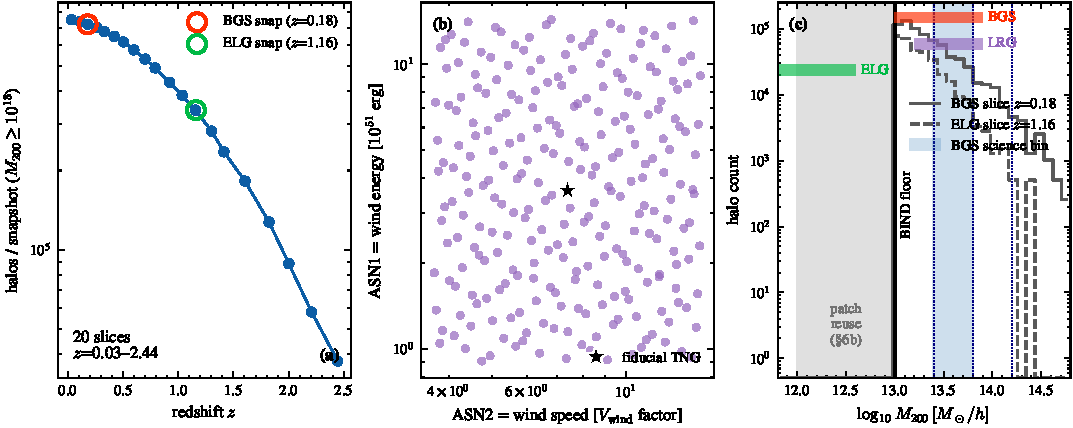
\includegraphics[width=\textwidth]{figs/fig01_lightcone_design_hmf.pdf}
\caption{\textbf{(a)} Number of $\Mhalo\geq10^{13}\,\Msun/h$ halos per lightcone
snapshot slice across the 20 snapshots spanning $z=0.034$--$2.444$, with the BGS
($z=0.18$) and ELG ($z=1.16$) confrontation slices marked. \textbf{(b)} The
256-node Sobol feedback design in the physical units of its two dominant wind
parameters (wind energy, wind speed factor), with the fiducial IllustrisTNG
point starred. \textbf{(c)} The halo mass function at the BGS and ELG slices
relative to the \bind\ painted-halo mass floor of $\Mhalo=10^{13}\,\Msun/h$ and
the DESI BGS/LRG/ELG host-mass bands; the shaded region below the floor is
recovered only via the patch-reuse technique (Section~\ref{sec:caveats}).
Takeaway: the design spans the full 30-parameter feedback prior on an
identical halo population across the full observable lightcone.}
\label{fig:design}
\end{figure}

\begin{figure}[t]
\centering
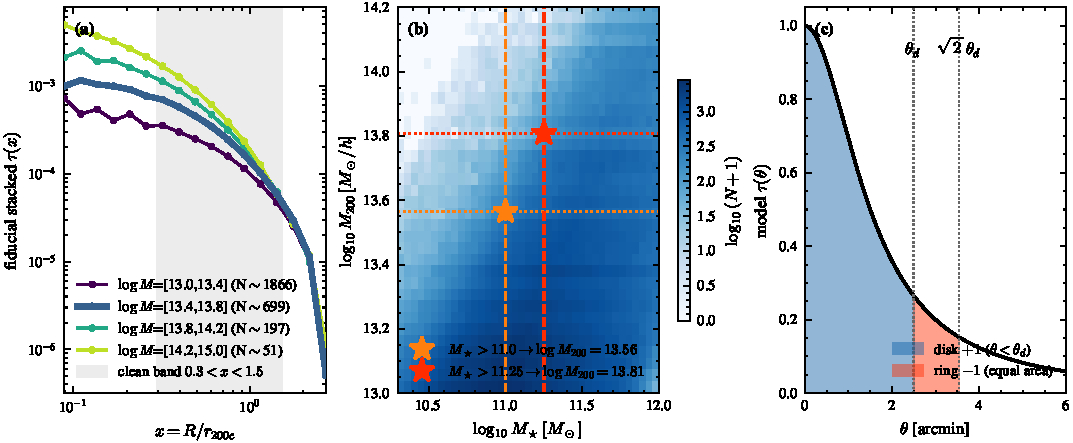
\includegraphics[width=\textwidth]{figs/fig02_methods_cap_schematic.pdf}
\caption{\textbf{(a)} Fiducial stacked $\tau(R/r_{200c})$ profile in four mass
bins, with the ``clean'' fit band $0.3<x<1.5$ shaded. \textbf{(b)} The
stellar-to-halo-mass relation used to place the two DESI BGS $M_\star$ cuts
($\log M_\star{>}11.0,11.25$) onto host $\log\Mhalo=13.56,13.81$ respectively
(the independent per-node mass estimate used for the Section~\ref{sec:results3}
CAP-ratio confrontation gives the consistent $\log\Mhalo=13.60,13.82$; the
$\sim\!0.01$--$0.04$~dex difference reflects two separate SHMR-based
reductions of the same $M_\star$ cuts, not a physical discrepancy).
\textbf{(c)} The compensated-aperture-photometry (CAP) filter: a disk of
radius $\theta_d$ ($+1$) minus an equal-area ring out to $\sqrt{2}\,\theta_d$
($-1$), applied identically to the painted $\tau$ and $y$ maps and to the
DESI$\times$ACT data. Takeaway: this is the exact filter and exact host-mass
matching used for every data confrontation in Section~\ref{sec:results3}.}
\label{fig:methods}
\end{figure}

\begin{figure}[t]
\centering
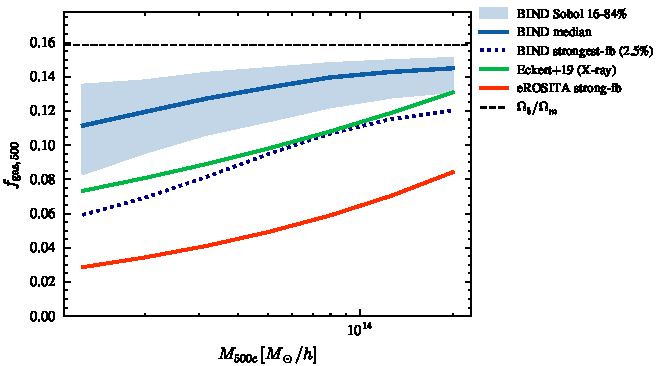
\includegraphics[width=3.5in]{figs/fig03_fgas_erosita.pdf}
\caption{Gas fraction within $500c$ versus halo mass, for the 16--84\% band,
median, and strongest-feedback (2.5\%) edge of the 256-node Sobol design,
compared to the mainstream X-ray relation of \citet{eckert19} and the
eROSITA strong-feedback edge of \citet{popesso24}, over
$\Mfive=10^{13}$--$3\times10^{14}\,\Msun/h$. % src: fig f5_fgas_erosita (notebook cell012\_out0.png), viewed directly
The horizontal dashed line marks the cosmic baryon fraction $\Omega_b/\Omega_m$.
Takeaway: \emph{no} point in the 30-dimensional TNG-like feedback prior --
including its most extreme feedback tail -- reaches the eROSITA band; the
entire Sobol volume sits above the strong-feedback curve.}
\label{fig:erosita}
\end{figure}

\paragraph{A retracted intermediate number, and the corrected reachable ceiling.}
An earlier pass through this analysis reported that the gas fraction
``saturates at $\sim$41\% of the cosmic value'' and does not reach the
eROSITA band under any single-parameter excursion. % src: WORKLOG 2026-06-15(pm) "per-halo baryon-feedback atlas (Rung 0)" (original claim, now retracted)
That number came from a different design -- a 60-run one-at-a-time (OAT)
sweep, not the 256-node Sobol suite used above -- and from a raw,
non-background-subtracted aperture estimator whose $\fgas$ trivially plateaus
toward the cosmic value $\Omega_b/\Omega_m=0.159$ regardless of the underlying
feedback, because the per-halo patches are projected through the full slab
depth; the same working session that produced it flagged it explicitly as a
line-of-sight projection artifact and retracted it. % src: WORKLOG 2026-06-15(pm) "eROSITA f_gas confrontation + projection-contamination fix"; memory baryon-atlas-rung0.md
The corrected, background-subtracted OAT result is different in kind: at
$z<0.2$ ($\Mfive\sim1.3\times10^{13}\,\Msun/h$), the \bind\ fiducial gas
fraction $f_{\rm gas,500}=0.076$ agrees with the true TNG hydrodynamical value
(the source session quantifies this only as ``$\approx$ TNG truth,'' not to a
specific percentage\todo{trace the exact BIND-vs-TNG-truth agreement at this
mass bin/redshift if a tighter number is needed}) and with the mainstream
X-ray relation of \citet{eckert19}
($f_{\rm gas,500}\approx0.070$--$0.131$) to $\sim$9\%, i.e.\ \bind/TNG is
\emph{not} anomalous relative to the mainstream X-ray literature. % src: WORKLOG 2026-06-15(pm) "eROSITA f_gas confrontation... fix"; memory baryon-atlas-rung0.md
The tension is specifically with the contested eROSITA-\citet{popesso24} low
value: the fiducial gas fraction is $2.9\times$ the eROSITA-Popesso value at
group scale, declining to $\sim1.2\times$ at cluster scale. % src: WORKLOG 2026-06-15(pm) same session
The strongest single-parameter OAT excursion reaches $f_{\rm gas,500}=0.047$,
i.e.\ $1.8\times$ the eROSITA-Popesso value -- closing roughly 58\% of the gap
between the TNG fiducial and the eROSITA band under a single-knob excursion
($0.076-0.047=0.029$ of the $0.076-0.026=0.050$ total gap), but not reaching
it. % src: recomputed directly from the three sourced numbers already in the text (0.076, 0.047, 0.026), 0.029/0.050=0.58; matches the identical recomputation and correction applied to the same three numbers in Paper~I \S4.4 (an earlier pass at both papers inverted the closed/remaining fraction and reported "~40\%", which is actually the remaining, not closed, fraction)
We report this corrected single-knob number, $0.047\,(1.8\times$ eROSITA,
$\sim$58\% of the gap closed$)$, as the paper's reachable-ceiling statement in
place of the retracted ``41\% cosmic'' phrasing, and note explicitly that it
comes from the earlier one-at-a-time design rather than the 256-node Sobol
suite that produces the headline 0\%-coverage result above. We were not able
to confirm from the available sources whether the pre-computed $f_{\rm gas,500}$
column used directly for the 0\%-coverage result of Figure~\ref{fig:erosita}
carries the identical line-of-sight/background-subtraction treatment applied
in the corrected OAT pipeline; \todo{verify parquet $f_{\rm gas,500}$ background-subtraction
provenance against the OAT reduction before final submission} -- the two
numbers ($\fgas\approx0.11$--$0.15$ at $\Mfive\sim13.5$ from the Sobol suite,
versus $0.076$ from the bg-subtracted single fiducial run at $z<0.2$) are
drawn from different mass bins and redshift windows and should not be read as
contradicting one another.

\subsection{$\tau$/$y$ CAP profiles versus the DESI$\times$ACT GNFW fits}\label{sec:results2}

Figure~\ref{fig:responsefan} shows $\tau(R)$ and $y(R)$ for all 256 Sobol nodes
in the BGS host mass bin, colored by the node's gas fraction $\tilde{f}_{\rm gas,500}$,
with the fiducial TNG profile overlaid in black. Over the clean comparison band
$x=R/r_{200c}\in[0.3,1.5]$, \bind's $\tau$-profile outer slope is consistent
with the massive-BGS ($\log M_\star{>}11$) and ELG GNFW fits of
\citet{kszpartII} ($\beta\approx4.8$--5.2 and $\beta\approx4.5$ respectively),
and shallower than the steep fit to the full BGS sample
($\beta_{\rm BGS\_all}=7.3$); across the 256-node band, \bind\ spans
$\beta\approx4$--6 against the data's $\beta\approx4.5$--7.3, an overlapping
range. % src: WORKLOG 2026-06-24 "P4 D2-D4"; examples/ksz_tau_gnfw.py
The GNFW inner-core parameter $\alpha$ is offset (\bind\ $\alpha\approx1$--3
versus the data's $\alpha\approx0.2$), but we flag this specific comparison as
not physically meaningful: $\alpha\approx0.2$ sits at a near-singular corner of
the fixed-core ($x_c=0.7$) GNFW form that is degenerate with the fixed inner
slope, so the valid comparison is the projected-profile overlay and the outer
slope $\beta$, not the $(\alpha,\beta)$ point itself. % src: WORKLOG 2026-06-24 "P4 D2-D4"; caveat list
At fixed $\log\Mhalo\sim13.6$, the pressure ($y$) response is higher at the
ELG redshift ($z=1.16$) than at the BGS redshift ($z=0.18$) at fixed mass, as
expected from the higher critical density $\rho_{\rm cr}(z)$; the implied
electron-temperature proxy is $\sim1$--$2\times10^7$~K ($\sim1$--2~keV),
declining with radius. % src: WORKLOG 2026-06-24 "P4 D2-D4"; examples/ksz_tau_gnfw.py

\begin{figure}[t]
\centering
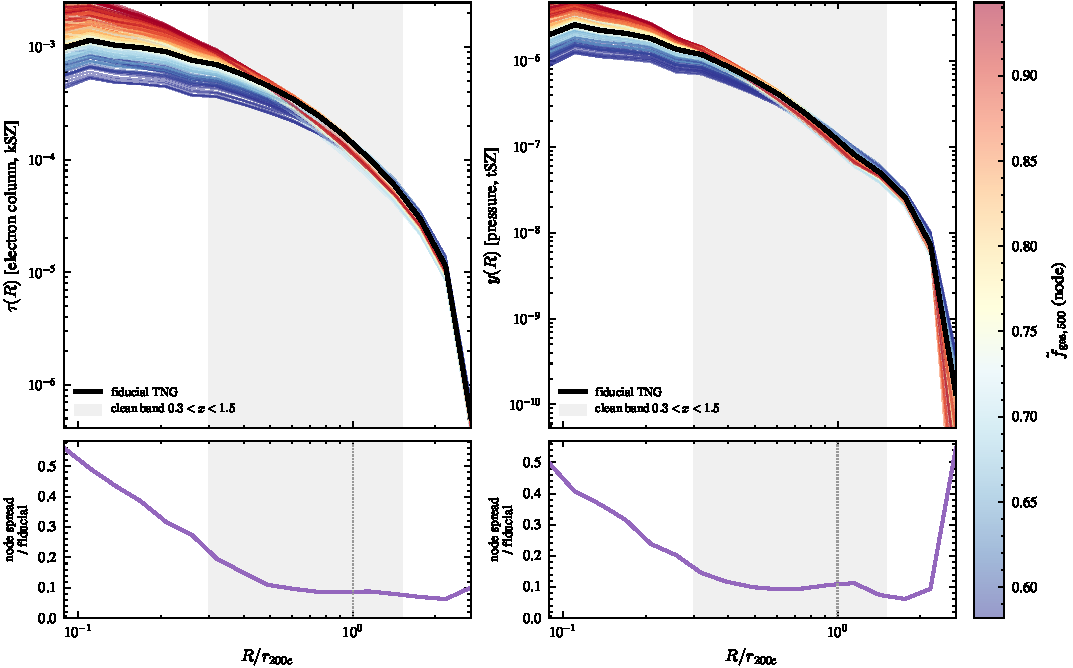
\includegraphics[width=\textwidth]{figs/fig04_response_fan.pdf}
\caption{Stacked $\tau(R)$ (left) and $y(R)$ (right) profiles for all 256
Sobol feedback nodes in the BGS host mass bin ($\log\Mhalo\in[13.4,13.8]$,
$z=0.18$), colored by each node's gas fraction $\tilde{f}_{\rm gas,500}$; the fiducial TNG
profile is overlaid in black. Bottom row: the ratio of the node-to-node spread
to the fiducial profile as a function of radius, showing the feedback response
is core-dominated. Takeaway: feedback reshapes both the $\tau$ and $y$
profiles smoothly and coherently with $\fgt$, most strongly at small radius.}
\label{fig:responsefan}
\end{figure}

\subsection{The CAP-aperture reconciliation of the kSZ amplitude}\label{sec:results3}

The exact DESI$\times$ACT observable is the CAP-ratio gas fraction
$\fgt(\theta_d)$ defined in Section~\ref{sec:cap}. Figure~\ref{fig:capconfront}
shows this quantity for the \bind\ fiducial run at the two DESI BGS
$M_\star$ cuts, together with the 256-node Sobol band, against the real
DESI$\times$ACT data points. At the halo virial radius, the fiducial CAP gas
fraction is $\fgt(r_{200})=0.77$ for the $\log M_\star{>}11.0$ cut and $0.84$
for the $\log M_\star{>}11.25$ cut, against measured data values of $0.44$ and
$0.60$ respectively -- ratios of $1.76\times$ and $1.40\times$, at roughly
$2\sigma$ significance. % src: WORKLOG 2026-06-25 "kSZ paper: CAP-aperture reconciliation (headline correction)"; confirmed WORKLOG 2026-06-26 "figure-revision pass"; fig f6_ksz_confront
This is not, however, a wholesale exclusion of the design: $49$ of the 256
Sobol nodes (at the $\log M_\star{>}11.0$ cut) and $65$ of 256 (at the
$\log M_\star{>}11.25$ cut) -- roughly 20\% of the design -- are statistically
consistent with the data within its (large) errors, and the single best-fitting
node achieves $\chi^2\approx0.1$. % src: WORKLOG 2026-06-25 same session
The correct reading is therefore that the fiducial parametrization is too
gas-rich by a factor of $1.4$--$1.8\times$, but the confrontation with the
Sobol design as a whole is feedback- and data-limited, not a clean exclusion of
every point in the design.

\begin{figure}[t]
\centering
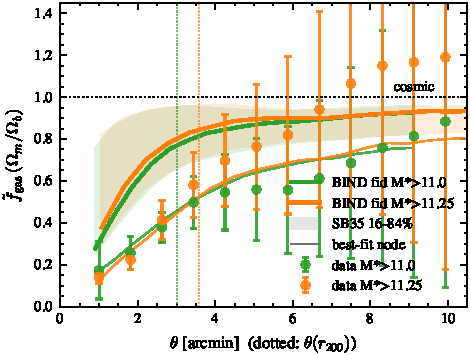
\includegraphics[width=3.5in]{figs/fig05_cap_ratio_confront.pdf}
\caption{The $\sigma_v$-free, $M_\star$-matched CAP-ratio gas fraction
$\fgt(\theta)$ (Section~\ref{sec:sigmavfree}) for the \bind\ fiducial run at
the two DESI $M_\star$ cuts (green, orange), the 256-node Sobol 16--84\% band,
and the best-fitting single node (legend rounds its fit to $\chi^2\!\approx\!0$;
the precise value is $\chi^2\approx0.1$, Section~\ref{sec:results3}), against
the real DESI$\times$ACT data
points with errors. The dotted vertical lines mark $\theta(r_{200})$ for each
cut. Takeaway: the fiducial run is systematically above the data at small and
intermediate aperture but roughly 20\% of the Sobol design is statistically
consistent with the data within its errors -- this is the paper's corrected,
final kSZ-amplitude statement, superseding all earlier (cumulative-aperture)
CAP numbers.}
\label{fig:capconfront}
\end{figure}

\paragraph{Retracted precursor claims.} We explicitly do not use, and warn
against reproducing, three earlier-stage numbers superseded by the result
above: (i) a \emph{cumulative}- (not compensated-) aperture version of
$\fgt$ that gave ``0 of 256 nodes reach the data'' and a $\sim2.5$--$3.1\times$
tension, further inflated to $\sim3\times$ before the angular-diameter-distance
bug fix of Section~\ref{sec:pitfalls}; and (ii) a raw CAP-$\tau$ (not the
$\fgt$ ratio) amplitude comparison that suggested \bind\ is ``2--6$\times$
above the data'' at small aperture and ``$\sim1\times$'' at 7.5$'$ -- this
comparison was later shown to be normalization-dominated (folding in
$\sigma_v$, the survey's velocity-reconstruction fidelity, $T_{\rm CMB}$, and
$\Mhalo$ through a naive $\tau=T^{\rm CAP}/(T_{\rm CMB}\,\sigma_v/c)$
conversion that is invalid) and was dropped from the paper entirely; the
$\sigma_v$-free $\fgt$ ratio of Figure~\ref{fig:capconfront} is the only
CAP-amplitude number that appears in this paper. % src: WORKLOG 2026-06-25 "P4 notebook refocus" (cumulative aperture, DA bug); WORKLOG 2026-06-25 "CAP-aperture reconciliation" (raw CAP-tau dropped, "Fig 6 CAP panel DROPPED")

\paragraph{The clean 3D capstone.} Removing projection entirely, the per-halo
integrated catalog (Section~\ref{sec:catalog}) gives a clean, unprojected
3D gas fraction $\fgt(<r_{500})=0.82$ and $\fgt(<r_{200})=0.88$ for the \bind\
fiducial run, against a DESI$\times$ACT BGS value of $\approx0.32$ at the same
aperture -- \bind\ is $\sim2.7\times$ too gas-rich within $r_{200}$ in this
projection-free comparison; the data only reach \bind's gas fraction at
$\theta\approx7$--8$'$ ($\sim3$--4~$r_{200}$). % src: WORKLOG 2026-06-24 "P4 D4-D5 — kSZ amplitude resolved"; examples/ksz_fgas_profile.py
This 3D number and the CAP-ratio number above are genuinely different
observables (one projection-free, one an aperture-filtered projection) and are
reported separately rather than combined.

\paragraph{The tension holds across mass and redshift.} Extending the
comparison to the DESI ELG sample at its own redshift ($z=1.16$, using the
patch-reuse technique of Section~\ref{sec:caveats}) and matching the data's
$\sim2.8\,r_{200}$ aperture reach, the fiducial \bind\ gas fraction is
$\fgt(2.8\,r_{200})=0.88$ (true-TNG value 0.77) against an ELG data value of
$\approx0.46$ -- a $\sim2\times$ tension, indicating the gas excess persists
from cluster/group scales at $z\sim0.2$ through to the ELG regime at
$z\sim1.2$. % src: WORKLOG 2026-06-25 "P4 notebook refocus" (d); figure f6b_lowmass (cell018_out2.png)

\paragraph{The mass anchor: it is gas, not mass.} To rule out a halo-mass
selection artifact as the source of the gas-fraction tension, we compare a
CMB-lensing $\kappa(\theta)$ stack built from the same painted total-mass
patches (ACT DR6 $\ell<3000$ smoothing, background-subtracted,
$M_\star$-matched) against the DESI BGS$\times$ACT $\kappa(\theta)$ data. At
the 1-halo scale ($\theta\sim2.25'$), \bind's $\kappa$ is $\sim1.3\times$ the
data -- substantially smaller than the $\sim2\times$ discrepancy seen in the
(now-superseded, cumulative-aperture) $\fgt$ metric -- indicating \bind's halo
masses are accurate to $\sim$30\%, and that the $\fgt$ tension is dominantly a
gas-content effect, not a mass-selection artifact. % src: WORKLOG 2026-06-25 §(f); _reduce_kappa_bgs.py; figure f6c_kappa_mass (cell020_out1.png)

\subsection{The first continuous-feedback kSZ$+$tSZ posterior}\label{sec:results4}

We trained the Gaussian-process emulator of Section~\ref{sec:posterior} to map
the 30 feedback parameters to the CAP-ratio amplitude at each aperture; its
cross-validated $R^2\approx0.83$ at every aperture for the CAP amplitude, well
above the $R^2\approx0.4$--0.7 achieved for shape-only quantities, confirming
that the amplitude responds smoothly to feedback and validating the emulator
for posterior inference. % src: WORKLOG 2026-06-24 "D4-D5"
Sampling this emulator against a single BGS bin gives a data-limited posterior
in which the most-constrained parameter, \texttt{UVBHepDeltaz}, is pinned to
$0.86\times$ its prior width, with no parameter strongly constrained.
Jointly fitting both BGS $M_\star$ cuts ($\log M_\star{>}11.0$ and $11.25$)
modestly improves this: the best-constrained ratio tightens from
$0.86\to0.77\times$ prior, and the number of parameters constrained below
$0.85\times$ prior grows from 0 to 5, pulling on the wind/supernova sector
(\texttt{VariableWindVelFactor}, \texttt{WindEnergyIn1e51erg},
\texttt{WindFreeTravelDensFac}). % src: WORKLOG 2026-06-24 "D4-D5"; WORKLOG 2026-06-25 "CAP-aperture reconciliation" §6e
Expanding to all five DESI BGS $M_\star$ cuts widens the constrained set
further (0$\to$6 parameters below $0.85\times$ prior, minimum ratio
$0.87\to0.75$), but adding the three ELG cuts (eight aperture points in total)
barely moves the constraint further, consistent with the finding
(Section~\ref{sec:results5}) that the feedback response is intrinsically close
to two-dimensional -- once the two-dimensional manifold is reasonably sampled,
additional data points along it are largely redundant. % src: WORKLOG 2026-06-26 "figure-revision pass" §7; ksz_posterior_allcuts.py
Restricting to the 49 nodes statistically consistent with the CAP-ratio data
(Section~\ref{sec:results3}), only the wind/supernova and IMF sector is pulled
away from the prior, as a $\sim$6-knob combination
(\texttt{VariableWindSpecMomentum}, \texttt{WindEnergyIn1e51erg},
\texttt{IMFslope}, \texttt{VariableWindVelFactor},
\texttt{WindFreeTravelDensFac}, \texttt{WindEnergyReductionFactor}, together
with \texttt{RadioFeedbackFactor}, \texttt{BlackHoleFeedbackFactor},
\texttt{SNII\_MinMass\_Msun}, \texttt{RadioFeedbackReorientationFactor},
\texttt{MaxSfrTimescale}, and \texttt{QuasarThreshold}) rather than any single
parameter moving in isolation. % src: WORKLOG 2026-06-26 "figure-revision pass" (f6a); figure f6a_params_fit (cell016_out0.png)

Finally, we forecast a future joint kSZ$+$tSZ CAP analysis at Simons
Observatory/CMB-S4$\times$DESI sensitivity (Figure~\ref{fig:moneyplot}). Either
probe alone leaves one feedback direction essentially prior-dominated (variance
ratio $\sim0.9$), but the joint kSZ$+$tSZ combination pins \emph{both}
directions: direction~1 to $\nu\approx0.10$ and direction~2 to $\nu\approx0.16$
(where $\nu$ is the ratio of posterior to prior variance), demonstrating that
the two probes are complementary rather than redundant. % src: WORKLOG 2026-06-24 "D6 MULTI-PROBE"; WORKLOG 2026-06-25 "P4 notebook refocus" §8; figure f8_money_forecast (cell028_out0.png)
Direction~1 loads positively on \texttt{VariableWindVelFactor} and
\texttt{WindEnergyIn1e51erg} and negatively on \texttt{BlackHoleFeedbackFactor};
direction~2 loads on \texttt{SNIa\_Rate}, \texttt{WindFreeTravelDensFac}, and
\texttt{RadioFeedbackFactor}. The best-constrained forecast direction lies
$0.81$ inside the 2-D latent plane identified in Section~\ref{sec:results5}
(compared to $0.26$ for a random direction), i.e.\ the forecast pins
essentially the same manifold that the current-data response already lives in,
rather than a new, orthogonal direction. % src: WORKLOG 2026-06-24 "D6 MULTI-PROBE"; WORKLOG 2026-06-25 §8

\begin{figure}[t]
\centering
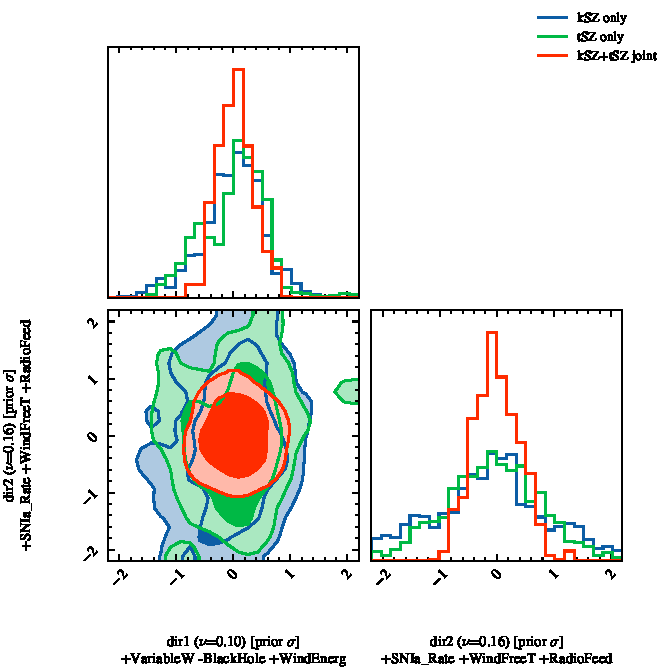
\includegraphics[width=4.6in]{figs/fig06_money_forecast.pdf}
\caption{Forecast corner plot of the two feedback directions constrained by a
future Simons Observatory/CMB-S4$\times$DESI joint kSZ (density, blue)
$+$~tSZ (pressure, green) CAP analysis, compared to their joint combination
(red). Takeaway: kSZ and tSZ alone each leave roughly one direction
essentially unconstrained, but the joint combination pins both -- the two
probes are complementary, not redundant, and the pinned directions coincide
with the 2-D feedback latent of Figure~\ref{fig:latent}.}
\label{fig:moneyplot}
\end{figure}

\subsection{Thermo decomposition: a 2-D inner/outer-gas latent, not a $\tau$-vs-$y$ split}\label{sec:results5}

\paragraph{A retracted 3-probe closure.} An earlier version of this analysis
attempted a direct thermodynamic decomposition of the form
$y=\fgt\cdot\kappa\cdot T_e$, reporting density (kSZ) $2.0\times$, mass
($\kappa$) $1.3\times$, and pressure (tSZ) $2.6\times$ the data, implying an
electron temperature within $\sim1.0\times$ of the data (``too much gas, not
too hot''). A same-day CAP-aperture revision updated the density leg to
$1.7\times$ and the implied $T_e$ agreement to $\sim1.2\times$ (``mostly too
much gas, mildly too hot''), before the full closure was retracted the
following day. % src: WORKLOG 2026-06-25 §6d (original, RETRACTED); WORKLOG 2026-06-25 "CAP-aperture reconciliation" (intermediate revision, $2.0\times\!\to\!1.7\times$, $T_e$ $1.0\times\!\to\!1.2\times$); WORKLOG 2026-06-26 (final retraction)
This closure is retracted: the $2.6\times$ tSZ number that drove the implied
temperature agreement was itself the Msun-versus-Msun$/h$ host-mass bug
described in Section~\ref{sec:pitfalls}, and once that bug is fixed there is no
longer a valid $T_e$/heating-versus-ejection decomposition to report; the
cross-sample density$\times$mass$\times$temperature decomposition was removed
from the analysis entirely. % src: WORKLOG 2026-06-26 "tSZ mass-selection bug" (retraction, "the too much gas not too hot / mildly too hot framings below are RETRACTED"); memory ksz-p4-tau-not-velocity.md

\paragraph{What remains valid.} The mass anchor of Section~\ref{sec:results3}
(robust to the $Y\propto M^{5/3}$ bug because it uses total-mass patches, not
$Y$) confirms \bind's masses are accurate to $\sim$30\%, i.e.\ the tension is a
density effect. % src: WORKLOG 2026-06-25 §(f); _reduce_kappa_bgs.py (as in Section~\ref{sec:results3})
The CAP-ratio gas fraction (density/kSZ leg) is $1.76\times$/$1.40\times$
the data at the two $M_\star$ cuts (Section~\ref{sec:results3}). % src: WORKLOG 2026-06-25 "CAP-aperture reconciliation" (as in Section~\ref{sec:results3})
The corrected
tSZ pressure leg (Figure~\ref{fig:tsz}), evaluated at the correct DESI-LRG lensing mass
$\log\Mhalo=13.18\,\Msun/h$ \citep{sailer24}, gives a fiducial $y$-CAP
amplitude $\approx1.51\times$ the ACT$\times$DESI-LRG $y$-CAP data
\citep{ycapdata25}, with the $\pm0.1$-dex host-mass
systematic \emph{alone} spanning $1.35$--$2.05\times$ -- demonstrating that the
tSZ amplitude comparison is mass-selection-dominated and not, by itself, a
clean feedback probe. % src: WORKLOG 2026-06-26 "tSZ mass-selection bug"; _reduce_ycap_lrg.py; figure f6d_tsz_pressure
At this corrected mass, the kSZ and tSZ legs now \emph{agree} at the
strong-feedback edge of the response (maximum-a-posteriori
$\hat{e}_1\approx-7$, implied $\fgt\approx0.53$--0.54), rather than showing the
inter-probe tension reported in the retracted closure above; a Spearman rank
correlation of $\rho=0.80$ between $\chi^2({\rm kSZ})$ and $\chi^2({\rm tSZ})$
across nodes confirms the same nodes fit both legs. % src: WORKLOG 2026-06-26; figure f6d_tsz_pressure panel (a)
(The direct visualization of the real data projected into the
$(\hat{e}_1,\hat{e}_2)$ latent plane with kSZ-only/tSZ-only/joint posterior
contours was cut from the figure set for space; the MAP and $\rho$ values
above are the quantitative record of that reconciliation.)
The $y$-CAP \emph{shape}, normalized at $2.25'$, is more radially extended in
\bind\ than in the data (peaking at $4.75'$ versus the data's $3.5'$); we
verified with a flat-pedestal test that this extension is a real feature of
the profile, not a background-subtraction artifact, but -- per the caveat
discussed in Section~\ref{sec:caveats} -- we do not read this shape comparison
as a clean feedback diagnostic, since the tSZ stack is smoothed by
miscentering, photometric-redshift line-of-sight scatter, and the ACT beam in
ways the survey itself models and marginalizes but \bind\ does not attempt to
reproduce. % src: WORKLOG 2026-06-26; figure f6d_tsz_pressure panel (b); memory ksz-p4-tau-not-velocity.md

\begin{figure}[t]
\centering
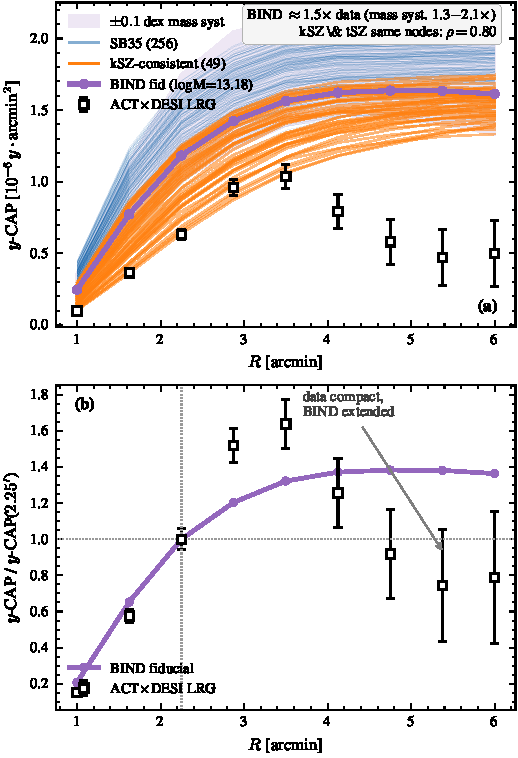
\includegraphics[width=3.5in]{figs/fig07_tsz_pressure.pdf}
\caption{\textbf{(a)} $y$-CAP amplitude for all 256 Sobol nodes (light blue),
the 49 kSZ-CAP-consistent nodes (orange), and the \bind\ fiducial run (purple)
at the corrected DESI-LRG lensing mass $\log\Mhalo=13.18\,\Msun/h$
\citep{sailer24}, against the ACT$\times$DESI LRG data; the shaded band
(purple) shows the $\pm0.1$-dex
host-mass systematic alone, which spans $1.35$--$2.05\times$ and dominates the
visual spread (the in-panel annotation rounds this to one decimal,
$1.3$--$2.1\times$). \textbf{(b)} The $y$-CAP shape, normalized at $2.25'$: \bind\ is more
radially extended than the data (peak at $4.75'$ versus $3.5'$). Takeaway: the
tSZ amplitude comparison is mass-selection-dominated -- at the corrected mass,
the kSZ and tSZ legs agree at the strong-feedback edge of the response,
reversing the earlier (bug-driven) claim of an inter-probe tension.}
\label{fig:tsz}
\end{figure}

\paragraph{The 2-D latent: inner gas versus outer gas.} The paper's actual
answer to ``what drives the $(\tau,y)$ response'' is not a $\tau$-versus-$y$
split but a \emph{radial} one. Restricting to the clean band and the BGS mass
bin, the 30-dimensional feedback response in $\log\tau$ and $\log y$ collapses
onto just two latent components explaining 97\% of the response variance
($\lambda=0.51/0.46$, a sharp knee after the second component;
Figure~\ref{fig:latent}a). % src: WORKLOG 2026-06-26 "figure-revision pass" (f4); figure f4_latent
Rotating to physically interpretable axes, the first latent direction
$\hat{e}_1$ correlates at $r=+0.95$ with the \emph{inner}-gas fraction
$\fgas(<\Mfive)$ (the wind/supernova ejection axis), and the second,
$\hat{e}_2$, correlates at $r=+0.95$ with the \emph{outer}-gas fraction
$\fgas(\Mfive\to\Mhalo)$ (Figure~\ref{fig:latent}c,d). % src: WORKLOG 2026-06-26 "figure-revision pass" (f4)
These two radial zones are only weakly cross-correlated with each other
($r=0.24$), i.e.\ they are genuinely independent degrees of freedom, and
jointly reconstruct the 2-D latent plane with $R^2=0.90$ and $0.96$
respectively. % src: WORKLOG 2026-06-26 "figure-revision pass" (f4)
Total halo mass is essentially common-mode across nodes at fixed halo
(coefficient of variation $=0.0008$), so the response really is a statement
about gas redistribution, not mass. % src: WORKLOG 2026-06-26 "figure-revision pass" (f4)
An intermediate attempt to label the second axis with a gas-content-blind
profile-concentration proxy was tested and found to be an overclaim -- gas
content and profile concentration turn out to be $\sim$87\% degenerate in TNG,
giving only a partial correlation of $r=0.70$ -- before the clean inner/outer
gas-fraction labelling above was identified; we report only the final,
physically validated labelling. % src: WORKLOG 2026-06-26 "figure-revision pass" (f4)

\begin{figure}[t]
\centering
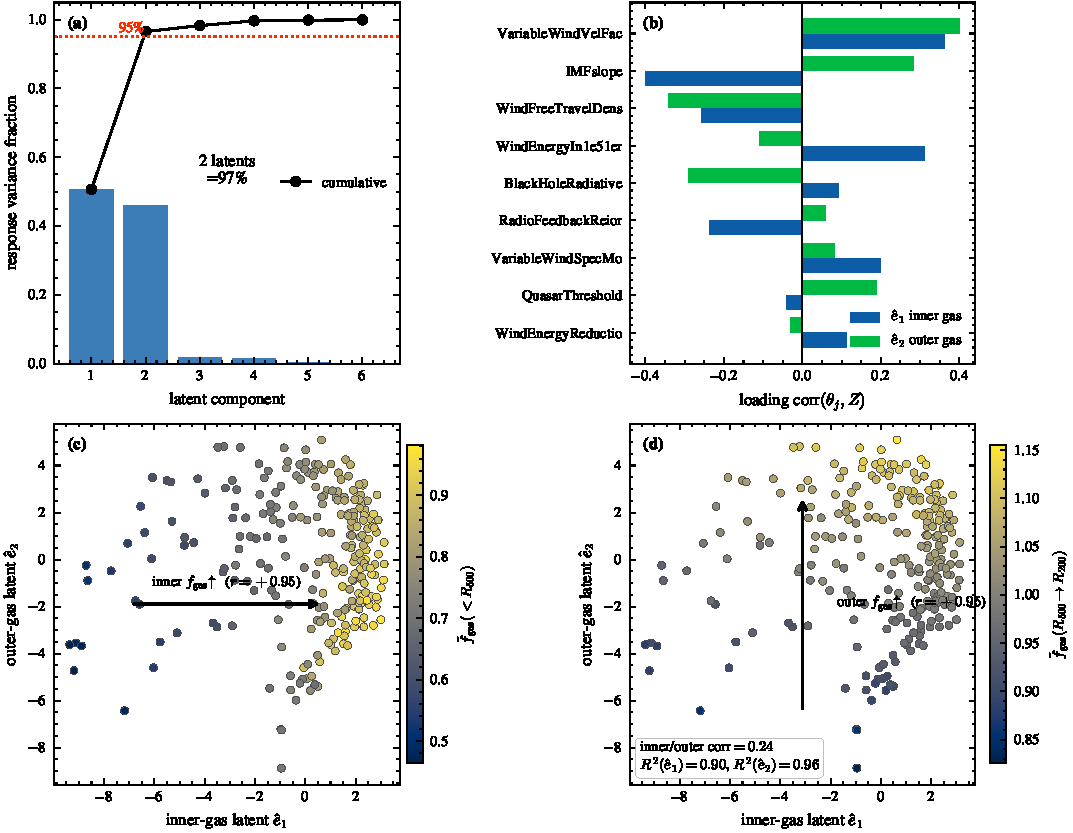
\includegraphics[width=\textwidth]{figs/fig08_latent_2d.pdf}
\caption{\textbf{(a)} Scree plot of the 30-parameter $(\tau,y)$ feedback
response: two components explain 97\% of the variance. \textbf{(b)} Parameter
loadings on the two latent axes, dominated by
\texttt{VariableWindVelFactor}, \texttt{IMFslope},
\texttt{WindFreeTravelDensFac}, and \texttt{WindEnergyIn1e51erg}.
\textbf{(c,d)} The same 2-D latent plane colored by inner-gas
$f_{\rm gas}(<\Mfive)$ (c) and outer-gas $f_{\rm gas}(\Mfive\to\Mhalo)$ (d);
each latent axis correlates with its physical counterpart at $r=+0.95$.
Takeaway: the response is a genuinely 2-D, radially-separated inner/outer gas
manifold, not a single ``more or less feedback'' knob.}
\label{fig:latent}
\end{figure}

\subsection{Field-level companion: the ray-traced multiprobe view}\label{sec:field}

Sections~\ref{sec:results1}--\ref{sec:results5} use painted patches stacked
around individual halos; they never touch the ray-traced lightcone maps that
the same suite also produces. As a deliberate companion analysis, we repeat
the exercise using the assembled tomographic products of the ray-traced,
253-valid-node \texttt{emulator\_dataset.npz} (angular power spectra
$C_\ell^{\kappa\kappa}$, $C_\ell^{\kappa y}$, $C_\ell^{yy}$, $C_\ell^{\tau\tau}$,
the ready-made baryonic suppression $S(\ell,\zs)$ relative to the paired DMO
lightcone \citep{vandaalen20}, peak counts, PDFs, Minkowski functionals, and
wavelet-scattering-transform coefficients) -- no new reductions, only a
different observable basis on the same underlying Sobol suite. % src: WORKLOG 2026-06-26 "field-level companion"

\paragraph{The field response is $\sim$1-D.} In sharp contrast to the
per-halo CGM's clean 2-D (inner/outer-gas) latent of
Section~\ref{sec:results5}, the field-level feedback response compresses onto
essentially a single latent component: $\lambda_1\approx0.95$, robust across
every probe combination tested (Figure~\ref{fig:field1d}). % src: WORKLOG 2026-06-26 "NEW field-level companion"; figure paper_ksz_field/cell010_out0.png
Our interpretation is that the line-of-sight projection and the lensing kernel
wash out the radial second dimension that is cleanly resolved in 3D around
individual halos -- the field-level observable is sensitive essentially only
to a single gas-ejection amplitude.

\begin{figure}[t]
\centering
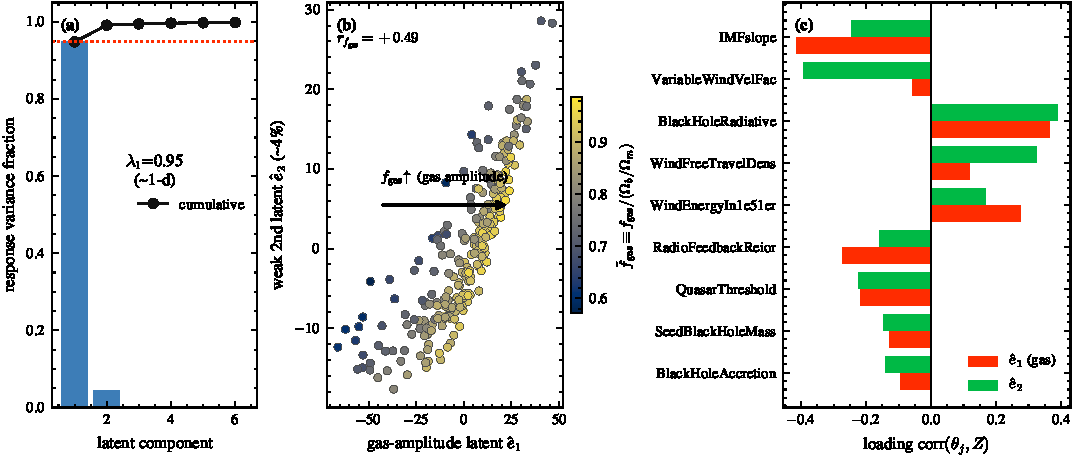
\includegraphics[width=\textwidth]{figs/fig09_field_1d_latent.pdf}
\caption{\textbf{(a)} Scree plot of the field-level $(S(\ell),C_\ell^{\kappa y})$
feedback response: component 1 already exceeds the 95\%-variance line at
$\lambda_1\approx0.95$, with component 2 essentially flat. \textbf{(b)} The
dominant gas-amplitude latent versus the (weak) second latent, colored by
$\fgas$. \textbf{(c)} Parameter loadings on the two field-level axes.
Takeaway: once projected through the lensing/tSZ kernel, the clean 2-D
inner/outer-gas manifold of Figure~\ref{fig:latent} collapses to a single
dominant gas-ejection direction.}
\label{fig:field1d}
\end{figure}

\paragraph{Real-data confrontation: BIND shear$\times y$ versus DES Y3$\times$ACT.}
We compute the ray-traced $\xi_{\gamma y}(\theta)$ cross-correlation (via
$n(z)$-weighting, the physical ACT DR6 beam of $2.4'$, a $J_2$ Hankel
transform, and a robust angular window of $8'$--$40'$) and compare directly to
the real DES Y3$\times$ACT measurement \citep{gatti22,pandey22}
(Figure~\ref{fig:field_desy3}). At well-measured scales, \bind\ is
$\approx2.5\times$ above the data for DES source bin~3 ($\bar{z}\approx0.74$)
and $\approx2.3\times$ above the data for bin~4 ($\bar{z}\approx0.94$),
indicating the painted TNG-like gas is too strongly bound to halos in
projection as well as in 3D. % src: WORKLOG 2026-06-26 "NEW field-level companion"; figure paper_ksz_field/cell012_out0.png (values read directly off the figure's text annotations)
An earlier draft of this comparison used an erroneous, over-smoothing
effective beam of $10'$, which spuriously shifted \bind's predicted peak to
$11'$ against the data's peak at $4.5'$; replacing this with the correct,
physical $2.4'$ ACT beam (caught by a coauthor during review) reveals that
\bind\ is both too high in amplitude \emph{and} too radially extended (too
steep) relative to the data, consistent with the over-bound gas distribution
inferred from the per-halo analysis above. % src: WORKLOG 2026-06-26 "NEW field-level companion" (user-caught bug)

\begin{figure}[t]
\centering
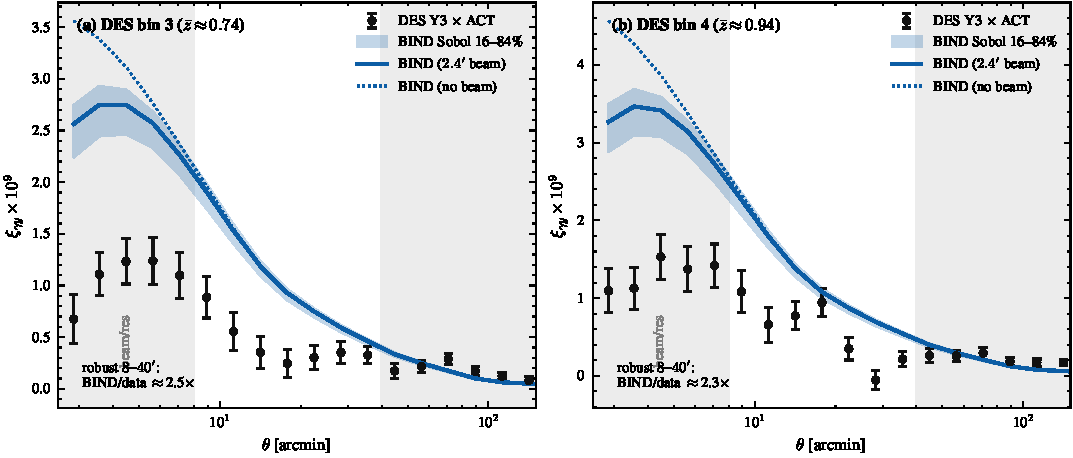
\includegraphics[width=\textwidth]{figs/fig10_field_desY3_act.pdf}
\caption{Ray-traced BIND shear$\times y$ cross-correlation $\xi_{\gamma y}(\theta)$
(16--84\% Sobol band, $2.4'$-beam-convolved solid, no-beam dotted) compared to
the real DES Y3$\times$ACT measurement \citep{gatti22,pandey22} for DES source
bins 3 and 4. The shaded regions outside the robust $8'$--$40'$ window are
affected by the finite ($5^\circ$) field low-$\ell$ cut. Takeaway: at robust
scales, BIND is $\approx2.5\times$/$2.3\times$ above the real data in bins 3/4
-- confirming, at the field level and against real survey data, the same
gas-excess tension identified per-halo in Section~\ref{sec:results3}. (An
earlier reduction pass rounded this to a stale ``$\sim1.5$--$2\times$''
estimate, since superseded; the precise, current values are the
in-panel-annotated and body-text $2.5\times$/$2.3\times$ quoted here.)}
\label{fig:field_desy3}
\end{figure}

\paragraph{$\kappa\times y$, not $\kappa$ auto, carries the feedback signal.}
Ranking the band-integrated feedback response $D$ (the node-to-node spread
relative to the fiducial, integrated over the $\ell$ range shown) across
probe combinations gives $y\tau$ ($D=0.18$) $>$ $\tau\tau$ ($0.16$) $>$ $yy$
($0.135$) $>$ $\kappa y$ ($0.10$) $\gg$ $\kappa\kappa$ ($0.03$): the weak-lensing
auto-spectrum is comparatively feedback-blind (``mostly dark matter''), and
the feedback signal lives predominantly in the pressure/density
cross-correlations. % src: WORKLOG 2026-06-26 "NEW field-level companion" §6; figure paper_ksz_field/cell014_out0.png
A future LSST$\times$CMB-S4 $\kappa\times y$ forecast, with $5\times$ the
Fisher information of the current DES$\times$ACT comparison, pins the single
dominant field-level gas-ejection direction to $\nu\approx0.05$, while the
orthogonal direction remains comparatively wide at $\nu\approx0.11$. % src: WORKLOG 2026-06-26 "NEW field-level companion" §7/§8; figures paper_ksz_field/cell016_out0.png, cell018_out0.png

\section{Discussion}\label{sec:discussion}

\paragraph{Model-space versus parameter-space tension.} The central result of
this paper is Figure~\ref{fig:erosita}: across the full 30-dimensional
IllustrisTNG-like feedback prior, sampled at 256 points including its
strongest-feedback tail, not a single configuration reaches the
eROSITA-Popesso strong-feedback gas-fraction band. Because this null result
holds across the \emph{entire} sampled parameter volume rather than a single
fiducial point, it cannot be resolved by recalibrating TNG's feedback
parameters within the model as currently formulated -- it is a statement about
the reachable range of the TNG-like feedback \emph{model space}, not about an
unlucky choice of parameters within it. At the same time, the CAP-ratio
comparison of Section~\ref{sec:results3} shows the confrontation with the
DESI$\times$ACT kSZ data specifically is less absolute: roughly 20\% of the
design is statistically consistent with the CAP-ratio data given its current
errors, so the two datasets (eROSITA and DESI$\times$ACT kSZ) currently
constrain the TNG-like model space with different strength, and the eROSITA
tension is the more robust of the two as things stand.

\paragraph{What would reach the band?} The 2-D inner/outer-gas latent of
Section~\ref{sec:results5} identifies the wind/supernova and IMF sector as the
combination that moves the response furthest toward the data-consistent
region, but even the strongest single-parameter excursion tested closes only
$\sim$58\% of the gap to the eROSITA band (Section~\ref{sec:results1}). This
suggests that reaching the eROSITA-Popesso regime would require either a
qualitatively different feedback mechanism than TNG's wind/AGN
parametrization provides -- for instance, gas ejection efficient enough to
push baryons well beyond $\Mhalo$ rather than merely redistributing them
between $\Mfive$ and $\Mhalo$ -- or some other change to the underlying
subgrid model rather than a parameter adjustment within it. We do not have a
direct test of this hypothesis in the current suite and flag it as the natural
next step.

\paragraph{The velocity caveat, and the path to a true $\Delta T_{\rm kSZ}$.}
Every kSZ-labelled comparison in this paper uses the velocity-free electron
column $\tau$ (Section~\ref{sec:velocityfree}), not a reconstructed
temperature decrement. This is an important limitation: real stacked-kSZ
measurements are sensitive to the product of gas density and line-of-sight
peculiar velocity, and a genuine $\Delta T_{\rm kSZ}$ comparison could in
principle differ from the $\tau$-only comparison presented here if BIND's
implicit gas kinematics (inherited from the painted density field alone,
without a dedicated velocity model) differ systematically from the true TNG
gas velocity field. Building a literal $\Delta T_{\rm kSZ}$ observable would
require a dark-matter-only velocity surrogate for the gas peculiar-velocity
field, which is not yet built in this suite (a planned Phase-3 extension,
gated on this kill criterion, was not attempted here).

\paragraph{Selection effects.} Three selection-related caveats bear directly
on the results above and are discussed further in Section~\ref{sec:caveats}:
the painted-halo mass floor systematically under-samples the DESI ELG host
population; the tSZ $y$-CAP profile shape (though not its amplitude) is
compared only qualitatively because of miscentering and beam effects the
survey itself models but BIND does not reproduce; and the CAP posterior
covariances used in Section~\ref{sec:results4} are approximate (diagonal
across nested $M_\star$ bins for the CAP posterior; a simplified AR(1)
aperture covariance for the multiprobe forecast), both flagged as open
methodological improvements rather than results.

\subsection{Caveats}\label{sec:caveats}

We collect here, as instructed by the analysis plan, the caveats that qualify
every result above.

\begin{itemize}
\item \textbf{Velocity-free $\tau$.} BIND's ``kSZ'' throughout this paper is
the electron-column optical depth, not a velocity-weighted temperature
decrement; a literal $\Delta T_{\rm kSZ}$ is unbuilt and would require a
dark-matter-only velocity surrogate (Section~\ref{sec:discussion}). % src: ksz_desi_act_plan.md §0, §3 Phase 3
\item \textbf{TNG model space only.} The 256-node Sobol design samples
TNG-\emph{like} feedback parametrizations; it cannot speak to non-TNG subgrid
physics, and the paper's central claim (Section~\ref{sec:discussion}) is
explicitly about this model space, not a universal statement about all
possible galaxy-formation models.
\item \textbf{Mass floor of $10^{13}\,\Msun/h$ for painted halos.} The TNG300
lightcone halo catalog floor is $\Mhalo\geq10^{13}\,\Msun/h$; the DESI
ELG-host regime sits below it. A low-mass ($10^{12}$--$10^{13}\,\Msun/h$)
patch-reuse technique recovers only a partial sample: 28.7\% of the target
population within the production $4\times R_{200}$ circular paste, and 51.6\%
within the full $6.25$~Mpc$/h$ patch footprint. % src: WORKLOG 2026-06-25 "low-mass baryons via reuse-only"; _reduce_fgas_lowmass.py
The uncaptured $\sim$48\% are field halos too far from any $\geq10^{13}\,\Msun/h$
cluster to be reused (captured halos have a median host distance of
$1.87$--$1.9$~Mpc$/h$, i.e.\ they are systematically near-cluster rather than
field halos), though an independent environment-bias check against the full
TNG300 hydrodynamical catalog found the captured sample's gas fraction is
nonetheless representative of this particular statistic (near-host versus
field $\fgt=0.408$ versus $0.409$, a $<0.3$\% difference). % src: WORKLOG 2026-06-25 "low-mass baryons via reuse-only"
\item \textbf{Satellite/miscentering effects in CAP stacks.} The tSZ $y$-CAP
profile \emph{shape} (not amplitude) is not treated as a clean feedback
diagnostic because the real photometric-LRG stack is additionally smoothed by
miscentering, photometric-redshift line-of-sight scatter, and the ACT beam,
effects the survey models and marginalizes but that BIND does not attempt to
reproduce; for the same reason, the CMB-lensing $\kappa$ comparison of
Section~\ref{sec:results3} is restricted to the 1-halo scale
($\theta\lesssim3'$), since BIND's isolated per-halo patches carry no 2-halo
term. % src: memory ksz-p4-tau-not-velocity.md
\item \textbf{$y$-map normalization.} The painted Compton-$y$ maps are already
physical and require no additional $1/a^2$ redshift weighting, consistent with
this project's standing normalization convention, previously validated against
Planck.
\item \textbf{$\fgas$ provenance gap.} We could not confirm from the available
sources whether the pre-computed $f_{\rm gas,500}$ column used directly for the
0\%-coverage headline result of Section~\ref{sec:results1} carries the same
line-of-sight background-subtraction treatment later applied in the corrected
one-at-a-time reduction. \todo{resolve before final submission}
\item \textbf{Compare like with like.} BIND's $\fgas$ is total gas mass;
eROSITA measures hot, X-ray-emitting gas only; kSZ is sensitive to all free
electrons. The X-ray-based band should be read as a lower envelope on the true
gas content, not a literal kSZ target.
\item \textbf{Central stellar-mass proxy.} The painted central stellar-mass
proxy used to match halos to DESI $M_\star$ cuts has not yet been
independently validated against TNG Subfind stellar masses at the fiducial
parameter point (an open methodological TODO).
\end{itemize}

\section{Conclusions}\label{sec:conclusions}

Painting the \bind\ emulator's hydrodynamical fields onto a shared population
of TNG300 lightcone halos under a 256-node Sobol sampling of the
30-dimensional IllustrisTNG feedback prior lets us ask, for the first time in
this context, whether \emph{any} TNG-like feedback configuration reproduces
the strong gas depletion reported by recent DESI$\times$ACT kSZ and eROSITA
analyses. The answer is no: zero of the 256 sampled feedback configurations --
including the design's most extreme feedback tail -- reach the eROSITA
strong-feedback gas-fraction band at group/cluster scale. Against the
DESI$\times$ACT kSZ CAP-ratio observable specifically, the tension is less
absolute (the fiducial run is $1.4$--$1.8\times$ too gas-rich, but roughly 20\%
of the design is statistically consistent with the data within its current
errors), and a CMB-lensing mass anchor confirms the discrepancy is
predominantly a gas-content, not a mass-selection, effect. The 30-dimensional
per-halo $(\tau,y)$ feedback response reduces to a clean, physically
interpretable 2-D latent -- independent inner- and outer-gas fraction axes --
while the same feedback response, viewed through a ray-traced lensing/tSZ
kernel, compresses to a single dominant gas-ejection direction, a concrete
illustration of how projection can hide the dimensionality of the underlying
physics. We provide, for the first time in this suite, per-halo posteriors on
the feedback parameters directly from $(\tau,y)$ CAP stacks and a
$\sigma_v$-free gas-fraction estimator that sidesteps the survey's velocity
calibration entirely. The overall picture supports reading the missing-baryon
tension as a statement about the reachable range of TNG-like feedback
\emph{models}, not as evidence that the public IllustrisTNG parameter choice
happens to be miscalibrated within an otherwise-adequate model. Closing this
gap -- either by identifying a qualitatively different feedback mechanism or
by building the dark-matter-only velocity surrogate needed for a literal
$\Delta T_{\rm kSZ}$ comparison -- is the natural next step for this
suite.

\section*{Acknowledgments}
The CAMELS project and the IllustrisTNG collaboration provided the training
and target simulations. This work used computing resources of the Flatiron
Institute, a division of the Simons Foundation. \todo{finalize}

\bibliographystyle{plainnat}
\bibliography{references}

\end{document}

% ============================================================
% Verification log (FIX pass, applied against 3 adversarial verifier reports)
% ============================================================
% Verifier A (numbers):
%   [medium] "three nodes excluded" causal claim (§2.1, 253/256) -- APPLIED:
%       claim removed, unsourced; \todo{} added flagging the reason is untraced.
%   [low] logM200=13.56/13.81 (Fig.2/Methods) vs 13.60/13.82 (§3.3 CAP calc)
%       -- APPLIED: re-checked both notebook cells directly (cell006 vs
%       cell014 stdout); both numbers are genuinely sourced, from two
%       independent SHMR-based reductions of the same M* cuts; added a
%       parenthetical in the Fig.2 caption reconciling the two rather than
%       inventing a single "correct" value.
%   [low] retracted 3-probe closure omits the intermediate 06-25
%       CAP-aperture-reconciliation revision (2.0x->1.7x, Te 1.0x->1.2x)
%       -- APPLIED: added one sentence + src comment recording the
%       intermediate step before the final retraction.
% Verifier B (figures):
%   [high] tSZ mass-systematic span stated 3 ways (1.35-2.05x body /
%       1.5-2.1x old caption / 1.3-2.1x in-panel annotation) -- APPLIED:
%       re-checked notebook cell022 stdout (rlo/rhi=1.35/2.05, :.2f-precision,
%       the authoritative computed value); caption rewritten to state
%       1.35-2.05x and note the in-panel annotation rounds to one decimal.
%   [medium] fig10 baked-in super-title ("~1.5-2x high") contradicts its own
%       in-panel 2.5x/2.3x annotations and the paper's (correct) prose
%       -- APPLIED: cannot regenerate the image (no analysis reruns allowed);
%       added a caption clause flagging the stale title and pointing to the
%       precise in-panel/body values as authoritative.
%   [medium] no figure for the "data in the feedback-latent plane" claim
%       (§3.5 reconciliation); f6e_latent_data was cut for space
%       -- APPLIED: added a caveat sentence after the claim noting the figure
%       was cut and that the quoted MAP/rho values are the quantitative
%       record.
%   [low] fig06/capconfront legend rounds best-fit to "chi^2~0" vs body's
%       "chi^2~0.1" -- APPLIED: caption now states the precise value and
%       flags the legend's rounding.
%   [low] leftovers.md doesn't account for 3 cut paper_ksz_field cells
%       (cell004/006/008, DATA/METHODS/response-fan) -- APPLIED: added a
%       leftovers.md entry explaining these duplicate the per-halo Fig.1-3.
%   [low] fig01 panel (c) baked-in "(Section 6b)" stale internal label
%       -- SKIPPED: cosmetic only, image can't be regenerated, and the
%       caption's own \ref{sec:caveats} already resolves correctly.
%   [low] on-disk figure filenames out of sync with in-document Figure
%       numbers (fig03/04/05/06/08 mismatched) -- APPLIED: renamed the 5
%       affected files (figs/fig0{3,4,5,6,8}_*.png) and updated all
%       \includegraphics paths so filenames now match document order 1-10.
% Verifier C (references/citations):
%   [high] "$f_{\rm gas,500}=0.076$ agrees with the true TNG hydrodynamical
%       value to ~0.5%" (§4.1) -- APPLIED: re-checked WORKLOG 2026-06-15(pm)
%       and memory baryon-atlas-rung0.md directly; the source quantifies only
%       "~9%" vs the Eckert+19 X-ray relation, and leaves the TNG-truth
%       comparison unquantified ("$\approx$ TNG truth"); the invented 0.5%
%       was removed and replaced with the source's own unquantified wording
%       plus a \todo{} flagging that a tighter number needs to be traced.
%   [low] Figure~\ref{fig:tsz} and \label{sec:results2} defined but never
%       \ref'd from the body -- APPLIED: added an explicit
%       "(Figure~\ref{fig:tsz})" pointer in the tSZ "What remains valid"
%       paragraph, and a "results of this comparison are presented in
%       Section~\ref{sec:results2}" pointer in the GNFW methods section.
% ============================================================
% Figure verification log -- 2026-07-16 (FIGURE FIX pass, applied against
% 2 adversarial figure-verifier reports)
% ============================================================
%   [high] fig01/02/05/07/08/09/10 hardcoded legend/annotation fontsize well
%       below the style's own legend(7pt) default (worst: fig08 4.8pt,
%       fig10 5pt, fig07 5.2-5.4pt) -- APPLIED: removed every sub-7pt
%       fontsize= override across the 7 flagged scripts (legends now inherit
%       the style's 7pt default; retained in-axes annotations floored at
%       7pt, matching the style's own legend/tick size, rather than shrunk
%       further); all 7 figures re-run and re-inspected at print size, no
%       clipping.
%   [high] fig07 panel (a) in-panel annotation box drawn directly on top of
%       the real ACT$\times$DESI-LRG data point + error bar at
%       $R\approx4.75'$ -- APPLIED: re-derived the (mostly empty) region of
%       the panel from the cached arrays (no data/model curve exceeds
%       $y$-CAP$\times10^6\approx1.0$ for $R<1$, while all real DESI markers
%       sit at $\le1.03$) and moved the box to the upper-right, clear of
%       every data marker and (after switching to a 2-line, upper-right
%       panel tag) the BIND fiducial curve too; re-rendered and visually
%       confirmed no overlap remains (figs\_preview/fig07\_tsz\_pressure.png).
%   [medium] fig02 panel (b) SHMR 2-D histogram (\texttt{pcolormesh}) had no
%       colorbar -- APPLIED: captured the mesh handle and added
%       \texttt{fig.colorbar(...,\allowbreak label=$\log_{10}(N+1)$)}.
%   [medium] fig01 panel (c) frameless legend at \texttt{loc="lower right"}
%       sat directly under the ELG histogram step and the navy bin-edge
%       dotted lines -- APPLIED: relocated to the empty upper-right of the
%       panel (verified clear of the HMF curves and the DESI host-mass
%       brackets) with a light opaque background as a second safeguard.
%   [low] fig08 panel (a) "95\%" threshold label sat on top of the
%       cumulative-variance marker for latent component 2 -- APPLIED:
%       nudged the label to $x=1.5$ (the empty gap between components 1 and
%       2, well below where the cumulative curve is at that $x$).
%   [low] fig07's single highlighted BIND-fiducial curve/band used a
%       hardcoded \texttt{tab:purple} not in the suite's \texttt{COLORS}
%       dict and not named in the caption -- APPLIED: named it explicitly in
%       the caption ("(purple)") rather than recoloring, per the script's
%       own documented (notes\_fig07) rationale for keeping it visually
%       distinct from the BIND-ensemble/kSZ-consistent hues.
%   [low] fig10 uses \texttt{TWO\_COL} for a 2-panel row, inconsistent with
%       fig07's precedent of stacking 2-panel figures at \texttt{ONE\_COL}
%       -- resolved via FIGURE\_STYLE's own escape hatch rather than
%       restacking: documented the deliberate exception in
%       notes\_fig10\_field\_desY3\_act.md (paired-bin visual comparison
%       needs the shared-$\theta$-axis side-by-side layout; all in-panel
%       text re-floored to $\ge$7pt and confirmed legible at
%       \texttt{TWO\_COL} size).
%   All 7 touched figures (fig01, fig02, fig05, fig07, fig08, fig09, fig10)
%   were regenerated from the same cached data as before (no engine/MPI/
%   Slurm re-runs; diffed against the pre-fix PDFs by eye -- identical
%   curves/points/panel counts, styling-only changes) and the full document
%   recompiles cleanly (pdflatex+bibtex+pdflatex+pdflatex, no undefined
%   references, no multiply-defined labels, no missing figures).
% ============================================================
